\documentclass[journal,10pt]{IEEEtran}
% UFUG2106 Stage 1 Technical Report — v1.0 references, visual hierarchy and supplementary tests.
% Compile from technical_report/: pdflatex main; bibtex main; pdflatex main x2
\usepackage[T1]{fontenc}
\usepackage{lmodern}
\usepackage{amsmath,amssymb,amsthm,mathtools}
\usepackage{graphicx,booktabs,array,tabularx}\usepackage{tikz}
\usetikzlibrary{arrows.meta,positioning,calc}
\usepackage{microtype}
\usepackage{balance}
\usepackage{url}
\usepackage{xcolor}
% Color specifications transcribed from the user's uploaded palette image (2026-11-11).
\definecolor{ResearchPeach}{HTML}{FAD6C9}
\definecolor{ResearchSage}{HTML}{B0C6A8}
\definecolor{ResearchIvory}{HTML}{FAF5E8}
\definecolor{ResearchBlue}{HTML}{92B3CD}
\definecolor{ResearchRose}{HTML}{D99DA3}
\definecolor{ResearchMint}{HTML}{D0E3DB}
\definecolor{ResearchSlate}{HTML}{A6B3C0}
\definecolor{ResearchStone}{HTML}{E8E2DB}

\usepackage{algorithm,algpseudocode}
\usepackage[hidelinks]{hyperref}
\newtheorem{theorem}{Theorem}
\newtheorem{lemma}{Lemma}
\newtheorem{proposition}{Proposition}
\newcommand{\AND}{\mathrm{AND2}}
\newcommand{\OR}{\mathrm{OR2}}
\newcommand{\NOT}{\mathrm{NOT}}
\newcommand{\arr}{\operatorname{arr}}
\newcommand{\area}{\operatorname{Area}}
\newcommand{\ddelay}{\operatorname{Delay}}
\newcommand{\Lset}{\mathcal{L}}
\begin{document}
\title{From Truth Tables to Timing-Constrained Gate DAGs:\\Representation, Global Sharing, and Evidence-Based Synthesis}
\author{Group 2 \\ Jincan LI jli843@connect.hkust-gz.edu.cn \\ Zeyun DU zdu881@connect.hkust-gz.edu.cn}
\markboth{UFUG2106 Stage 1: Truth Table to Circuit}{UFUG2106 Stage 1: Truth Table to Circuit}
\maketitle
\begin{abstract}
A complete truth table fixes Boolean behavior but leaves circuit structure, gate sharing, and timing unresolved. We study the construction of AND2/OR2/NOT netlists under case-specific area and delay costs, using an exact Shannon/ROBDD baseline, diversified mapping, required-time-aware recovery, and a more efficient synthesis engine. The frozen Round 5.1 research implementation passes all 25 released Stage 1 cases, meets every delay target, and achieves aggregate area 529,014. In two paired WSL comparisons with Round 5, median synthesis runtimes decrease from 72.188 to 55.488 ms and from 60.827 to 55.077 ms, with unchanged measured area and delay. A separate bounded cut-rewriting study discovers further area savings on released and generated functions but exceeds our prespecified synthesis-runtime tolerance. We report the distinction between functional proofs, implemented transformations, and empirical performance; neither minimum area nor performance on unreleased cases is claimed.
\end{abstract}
\begin{IEEEkeywords}
Logic synthesis, Shannon expansion, ROBDD, Boolean functions, technology mapping, timing analysis, combinational DAG, empirical reproducibility.
\end{IEEEkeywords}

\section{Introduction}
A complete truth table specifies behavior but not a circuit architecture. The simplest direct expression---for example a sum of minterms---can reproduce every table but duplicates intermediate predicates and may produce long logic paths. The practical problem is to construct a circuit that is not only correct but also inexpensive under the particular gate areas, delays and resource limits of each test case. This distinction between \emph{functional equivalence} and \emph{physical realization} is classical in switching-network synthesis~\cite{shannon1949,brayton1984}.

The released UFUG2106 Stage 1 task requires a single-threaded program that reads one complete table and emits a topologically ordered netlist using only three gate types. Its official evaluator reports pass/fail, area, circuit delay, synthesis runtime, and whether the circuit satisfies the designated delay target~\cite{coursehandout}. The numerical grading formula has not been published. We therefore do not equate aggregate area across the 25 published instances with a course score.

The central challenge is not to find one more Boolean identity. It is to decide \emph{which representation should be mapped, which gate structures should be shared, and which improvements justify the synthesis time spent discovering them}. This gives three linked research questions: \emph{(RQ1)} can an exact truth-table construction be diversified enough to satisfy the specified delay targets at lower area? \emph{(RQ2)} how should a shared, priced gate DAG exploit complements and timing slack without confusing local gate savings with global savings? \emph{(RQ3)} after circuit-quality gains become small, can the same search be made substantially cheaper, and do more expensive local rewrites warrant inclusion?

The development stages answer these questions in sequence rather than constituting independent features. Round 1 establishes an exact Shannon/ROBDD baseline, but its delay misses expose a representation problem. Round 2 widens the mapping portfolio. Round 3 shows that the \emph{mapped network}---not just the BDD---must be evaluated against global sharing and required time. Round 4 finds further area savings but makes additional search costly. Rounds 4.1--5.1 then focus on an efficiency-preserving implementation, before Rounds 6.0--6.1 deliberately test the value of an additional local rewrite family.

The contributions of this course-project study are \emph{(i)} a reproducible implementation combining established exact representations with case-dependent gate mapping and timing recovery; \emph{(ii)} an engineering refinement that reduces repeated synthesis computation while preserving measured circuit quality; and \emph{(iii)} evidence-backed adoption decisions that include a negative result for costly cut rewriting. These are integration and experimental contributions, \emph{not} claims to have invented ROBDDs, De Morgan transformations, or cut rewriting~\cite{bryant1986,mishchenko2006}. Every measured comparison below is explicitly attributed to its archive or paired experiment.


\begin{figure*}[!t]
\centering
% Editable two-column research architecture: no empirical quantities in this conceptual figure.
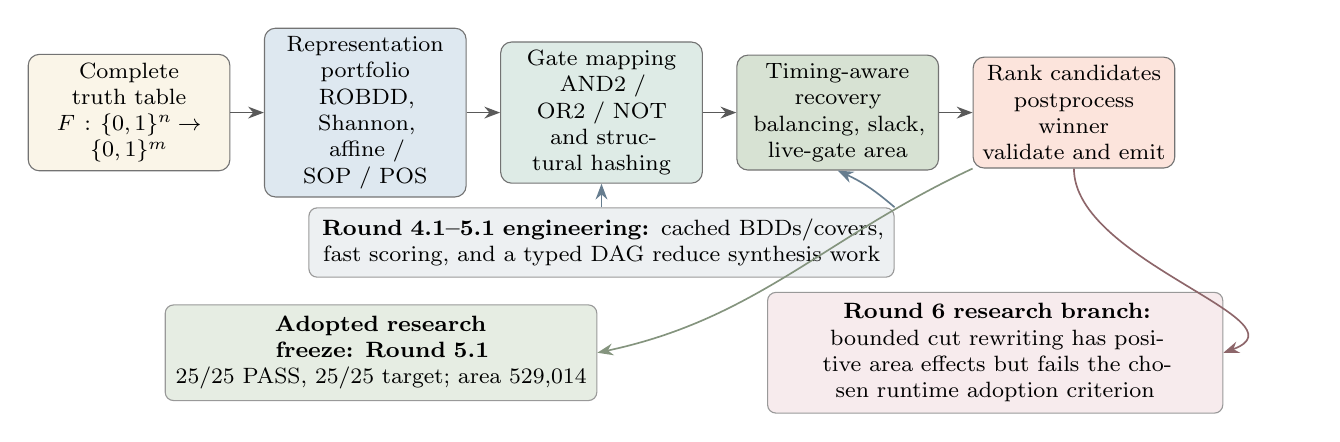
\begin{tikzpicture}[
 x=1cm,y=1cm,>=Stealth,
 every node/.style={font=\footnotesize},
 core/.style={draw=black!55,rounded corners=4pt,minimum height=11mm,text width=2.35cm,align=center,inner sep=3pt},
 band/.style={draw=black!40,rounded corners=3pt,text width=5.0cm,align=center,inner sep=4pt},
 arr/.style={-Stealth,semithick,draw=black!65}]
\node[core,fill=ResearchIvory] (input) at (0,0) {Complete truth table\\$F:\{0,1\}^n\!\to\!\{0,1\}^m$};
\node[core,fill=ResearchBlue!30] (repr) at (3.0,0) {Representation portfolio\\ROBDD, Shannon,\\affine / SOP / POS};
\node[core,fill=ResearchMint!70] (map) at (6.0,0) {Gate mapping\\AND2 / OR2 / NOT\\and structural hashing};
\node[core,fill=ResearchSage!50] (recover) at (9.0,0) {Timing-aware recovery\\balancing, slack,\\live-gate area};
\node[core,fill=ResearchPeach!65] (choice) at (12.0,0) {Rank candidates\\postprocess winner\\validate and emit};
\foreach \aa/\bb in {input/repr,repr/map,map/recover,recover/choice} \draw[arr] (\aa.east) -- (\bb.west);
\node[band,fill=ResearchSlate!20,text width=7.15cm] (eff) at (6.0,-1.65) {\textbf{Round 4.1--5.1 engineering:} cached BDDs/covers, fast scoring, and a typed DAG reduce synthesis work};
\draw[arr,ResearchBlue!70!black] (eff.north) -- (map.south);
\draw[arr,ResearchBlue!70!black] (eff.north east) to[bend right=8] (recover.south);
\node[band,fill=ResearchRose!20,text width=5.5cm] (cut) at (11.0,-3.05) {\textbf{Round 6 research branch:} bounded cut rewriting has positive area effects but fails the chosen runtime adoption criterion};
\node[band,fill=ResearchSage!32,text width=5.2cm] (frozen) at (3.2,-3.05) {\textbf{Adopted research freeze: Round 5.1}\\25/25 PASS, 25/25 target; area 529,014};
\draw[arr,ResearchRose!65!black] (choice.south) to[out=-90,in=20] (cut.east);
\draw[arr,ResearchSage!75!black] (choice.south west) to[out=-155,in=12] (frozen.east);
\end{tikzpicture}

\caption{Overview of the implemented Stage 1 synthesis workflow and the separately evaluated Round 6 research branch. Candidate-specific graph construction, balancing, and recovery precede winner selection; algebraic/phase postprocessing is applied to the selected incumbent, not to every portfolio member. BDD and implicant caching, fast scoring, and a typed DAG improve the main implementation's synthesis efficiency. Only legal AND2/OR2/NOT gates are emitted. The cut-rewriting branch remains experimental because its additional area gains did not justify its synthesis-runtime overhead.}
\label{fig:workflow}
\end{figure*}

\section{Formal Problem and Evaluation Contract}
Let $F:\{0,1\}^{n}\rightarrow\{0,1\}^{m}$ be the multi-output function represented by the complete truth table, where $1\le n\le18$ and $m\ge1$. Input vector $x=(x_0,\ldots,x_{n-1})$ indexes rows with $x_0$ most significant. The target network is a directed acyclic graph $G=(V,E)$ with source nodes for the constant zero and the $n$ primary inputs. Every remaining node is one of $\Lset=\{\AND,\OR,\NOT\}$; every output references a previously defined signal. Fanout and sharing are permitted.

For type $t\in\Lset$, let $a_t>0$ and $d_t>0$ be the given integer area and delay. With $N_t(G)$ denoting the number of \emph{emitted} gates of type $t$, the exact output-file area is
\begin{equation}\label{eq:area}
 A(G)=\sum_{t\in\Lset}N_t(G)a_t.
\end{equation}
We remove dead gates before emitting the network, so the charged set equals the live reachable subgraph. For any node $v$, define its arrival time recursively:
\begin{equation}\label{eq:arrival}
 T(v)=\begin{cases}
 0, &v\text{ source},\\
 T(u)+d_{\NOT}, &v=\NOT(u),\\
 \max\{T(u),T(w)\}+d_t, &v=t(u,w).
 \end{cases}
\end{equation}
Here $t\in\{\AND,\OR\}$ for binary gates. The network delay is $D(G)=\max_{j<m}T(y_j)$. The optimization is constrained by $G(x)=F(x)$ for every assignment, the legal-netlist format, the optional program runtime and RAM caps imposed by the evaluator, and preferably $D(G)\le D_{\rm target}$. Importantly, the course specification says that a functionally correct circuit can \emph{pass} while exceeding the target; a target miss carries a score penalty rather than necessarily implying invalidity. We report both metrics separately.

The provided Linux evaluator exposes additional command-line caps \texttt{--timeout-ms} and \texttt{--ram-kb}, and produces case-level validity and timing results. Neither its public interface nor the supplied instructions disclose a numerical grading formula. Our internal ranking in (\ref{eq:rank}) is therefore \emph{not} presented as an official score. The frozen program reads the optional runtime-limit value but does not explicitly parse or enforce the ninth-line RAM-limit value; published-case success is not a guarantee for every future memory cap.

A primary constraint is informational: the input already contains $m2^n$ truth bits, so merely reading the instance requires $\Omega(m2^n)$ bit operations in a conventional bit-level model. All our representations remain potentially exponential in $n$ in the worst case, even if typical functions admit compact shared DAGs.

\section{From Shannon Expansion to Shared Decision DAGs}
\subsection{An exact constructive baseline}
For any variable $x_i$, the cofactors $f_{i,0}$ and $f_{i,1}$ are the restrictions of $f$ with $x_i=0$ and $x_i=1$. By distinguishing these two cases,
\begin{equation}\label{eq:shannon}
 f=(\neg x_i\land f_{i,0})\lor(x_i\land f_{i,1}).
\end{equation}
This identity gives a constructive proof that every Boolean output can be expressed with $\AND$, $\OR$, and $\NOT$. It also supplies a recursive algorithm, but naïve recursion can repeat the same subfunction many times. Crucially, the identity fixes the value of the parent, not the number, shape, or price of physical gates used to implement it. An abstract decision node may resemble a two-input multiplexer, but a multiplexer is not included in the permitted library: an ordinary realization needs the appropriate input inversion, two conjunctions, and one disjunction. These gates can be reused across nodes, so multiplying a decision-node count by this naive per-node cost is generally incorrect.

For a fixed variable permutation $\pi$, an ROBDD interns every nonterminal decision node by $(\pi(k),\ell,h)$ and deletes a node when $\ell=h$. A unique table shares recurring cofactors between branches and output functions. Such ordered reductions preserve the represented function and give a canonical graph relative to the fixed order under standard assumptions~\cite{bryant1986}. The resulting decision graph is subsequently \emph{mapped} into permitted physical gates; a BDD node is not itself a free multiplexor. The distinction between \emph{functional} and \emph{syntactic} sharing is important: a gate-level structural hash can merge identical tuples $(\operatorname{op},a,b)$, but by itself cannot recognize that $(a\land b)\lor(a\land c)$ is functionally equal to $a\land(b\lor c)$. Such equalities require rewriting or a function-level representation. Hence a canonical ROBDD under one fixed order does not imply a minimum-area mapped circuit.

\begin{lemma}[Correctness of the baseline]
If each BDD terminal represents its Boolean constant, each nonterminal represents the function in (\ref{eq:shannon}), and its gate mapping uses exact AND/OR/NOT identities, then each emitted output equals its specified truth-table column.
\end{lemma}
\begin{IEEEproof}
Induct on the remaining decision levels. Terminals are exact. Assuming both child cofactors are exact, substitute them into (\ref{eq:shannon}); the result equals the parent for both possible values of the decision variable. The recursive mapping implements this expression with legal gates. Structural hashing replaces duplicated nodes only with equal functions, and dead-gate removal deletes only signals not reaching an output. Repeat for all $m$ roots.
\end{IEEEproof}

Round 1 validated this construction on all 25 published cases but met only 12 target delays. The failure mode is informative: Shannon's identity certifies \emph{which function} is computed, but says nothing about \emph{which graph shape} will meet a deadline. This observation justifies retaining the proof-producing decomposition while treating representation and gate mapping as optimization variables in Round 2.

\subsection{A small multi-output example}
Let the primary inputs be $a,b,c$ and the outputs be $f_1=(a\land b)\lor(\neg a\land c)$ and $f_2=f_1\lor b$. Shannon cofactors at $a$ give $(f_1|_{a=0},f_1|_{a=1})=(c,b)$ and $(f_2|_{a=0},f_2|_{a=1})=(b\lor c,b)$. The cofactor $b$ is shared, while sharing the \emph{physical} gate for $f_1$ is a separate mapping choice. With primary IDs $1=a,2=b,3=c$ and ID $0$ the constant zero, one legal topological construction is
\begin{equation*}
\begin{aligned}
4&=\NOT(1), &5&=\AND(1,2),\\
6&=\AND(4,3), &7&=\OR(5,6),\\
8&=\OR(7,2), & (y_1,y_2)&=(7,8).
\end{aligned}
\end{equation*}
For illustrative gate areas $(a_\AND,a_\OR,a_\NOT)=(2,3,1)$ and delays $(d_\AND,d_\OR,d_\NOT)=(2,2,1)$, this circuit has $A=11$, $T(7)=5$ and $T(8)=7$. Boolean absorption gives $f_2=b\lor(\neg a\land c)$, so replacing gate $8$ by $\OR(2,6)$ retains the same charged gate count but changes the second output arrival from $7$ to $5$. The example is a \emph{constructed illustration}, not one of the 25 benchmark inputs. It demonstrates why Boolean equality, shared-gate area and critical-path timing are three separate questions.

\begin{figure}[!t]
\centering
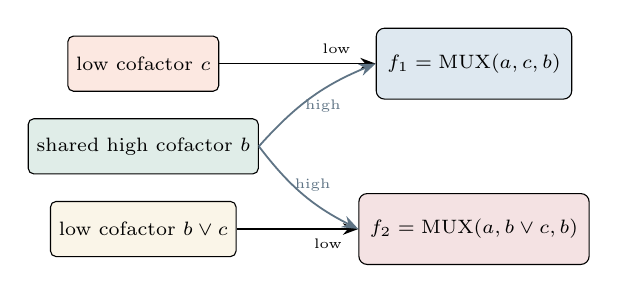
\begin{tikzpicture}[>=Stealth, x=1cm,y=1cm,
  every node/.style={font=\scriptsize},
  cnode/.style={draw,rounded corners=2pt,minimum height=7mm,align=center,inner xsep=3pt},
  outputbox/.style={draw,rounded corners=3pt,minimum height=9mm,align=center,inner xsep=4pt}]
\node[cnode,fill=ResearchPeach!55] (c) at (0,1.05) {low cofactor $c$};
\node[cnode,fill=ResearchMint!65] (b) at (0,0) {shared high cofactor $b$};
\node[cnode,fill=ResearchIvory] (bc) at (0,-1.05) {low cofactor $b\lor c$};
\node[outputbox,fill=ResearchBlue!30] (f1) at (4.2,1.05) {$f_1=\mathrm{MUX}(a,c,b)$};
\node[outputbox,fill=ResearchRose!30] (f2) at (4.2,-1.05) {$f_2=\mathrm{MUX}(a,b\lor c,b)$};
\draw[->,line width=.57pt] (c.east) -- node[above,near end,font=\tiny] {low} (f1.west);
\draw[->,line width=.57pt] (bc.east) -- node[below,near end,font=\tiny] {low} (f2.west);
\draw[->,line width=.65pt,ResearchBlue!65!black] (b.east) to[bend left=13] node[below,pos=.60,font=\tiny] {high} (f1.west);
\draw[->,line width=.65pt,ResearchBlue!65!black] (b.east) to[bend right=13] node[above,pos=.60,font=\tiny] {high} (f2.west);
\end{tikzpicture}
\caption{Two Shannon decompositions reuse the same high cofactor $b$; each output has a distinct low cofactor. The diagram shows functional dependence, not priced gate edges; the MUX is conceptual rather than an allowed physical primitive.}\label{fig:example}
\end{figure}

\subsection{Representation and candidate diversification}
ROBDD size, shared cofactors, and gate mapping depend strongly on variable order $\pi$. Round 2 introduced variable influence as an ordering heuristic, where for a single output
\begin{equation}
 I_i(f)=2^{-(n-1)}\sum_{x_{-i}\in\{0,1\}^{n-1}}
 \mathbf1\{f(x_{-i},0)\ne f(x_{-i},1)\}.
\end{equation}
For multiple outputs, the implementation combines observed variable effects when constructing its order. Influence is not a proof of the optimal order: even the smallest ROBDD need not map to the smallest gate DAG under nonuniform costs. To see why this statistic is incomplete, the running example gives $I_a(f_1)=I_b(f_1)=I_c(f_1)=1/2$: changing the selector matters only when the two data inputs differ, while changing either data input matters only in its selected branch. Thus all three variables tie in influence despite playing different structural roles. Influence can guide a candidate order, but only completed mapping and full-DAG cost evaluation determine its merit.

The portfolio also uses a two-level decomposition. With root variable $x$ and potentially distinct second variables $u$ and $v$ in the $x=0$ and $x=1$ branches,
\begin{multline}\label{eq:twolevel}
 f=\neg x\land\big(\neg u\land f_{00}\lor u\land f_{01}\big)\\
 \lor x\land\big(\neg v\land f_{10}\lor v\land f_{11}\big).
\end{multline}
Balancing the branch computations changes gate critical paths without changing the Boolean function. For outputs of small essential support, SOP/POS candidates use prime implicants followed by a deterministic greedy cover. Every selected cube is an implicant, and the chosen cubes cover the full on-set; hence the cover is exact, although generally \emph{not minimum-area}. Formally, if selected cubes $c_j$ satisfy $c_j(x)\Rightarrow f(x)$ for all $x$ and $f(x)\Rightarrow\bigvee_j c_j(x)$, then the two implications prove $f=\bigvee_jc_j$ pointwise. For POS, one can instead cover the complement $\neg f$ and negate the resulting exact SOP. The \emph{cover selection} and its \emph{gate realization} are distinct: a greedy minimum-cover proxy need not minimize the final priced, shared AND2/OR2/NOT network. These alternatives allow the selector to measure completed circuits instead of betting on one representation. The Round 2 archive records 25/25 target-met cases and area $790{,}243$, compared with 12/25 and $1{,}103{,}455$ for the baseline. Yet a better candidate portfolio still leaves one structural limitation: a local cofactor or mapping choice does not know whether its output will be shared, complemented, or given slack by the \emph{rest of the network}. That is the motivation for global, timing-aware recovery in Round 3.

\section{Cost-Aware Gate Mapping and Timing Recovery}
The preceding section chooses among equivalent \emph{descriptions} of Boolean functions. This section instead asks about their \emph{joint realization}: a gate shared by two outputs is charged once, but its arrival affects every downstream consumer. Polarity, balancing, and required-time optimization therefore operate on the whole costed DAG, rather than independently minimizing each output expression.
\subsection{Complemented functions and affine recognition}
Round 3 uses complemented-edge BDD references. A reference consists of a node identity and one inversion bit; complements can therefore share a common normalized subgraph. This saves BDD construction and may expose mapping opportunities, but it does not declare a physical NOT to have zero cost. Each emitted inverter is still charged under (\ref{eq:area}).

A recognized affine function has the form
\begin{equation}
 f(x)=c\oplus\bigoplus_{i\in S}x_i,
\end{equation}
where $c\in\{0,1\}$. If the two children of a BDD decision satisfy $f_1=\neg f_0$, (\ref{eq:shannon}) reduces to $f=f_0\oplus x$. Since XOR is not in the permitted library, it is lowered with the exact identity
\begin{equation}
 a\oplus b=(a\lor b)\land\neg(a\land b).
\end{equation}
Whether this is an improvement depends on gate prices, available shared signals, and critical-path depth; the ordinary Shannon implementation remains an alternative.

\subsection{Required-time-driven area recovery}
A locally shorter path need not be globally necessary. For an already timing-feasible network, Round 3 propagates required arrival times from each output, initially setting $R(y_j)=D_{\rm target}$, then traverses gates in reverse topological order:
\begin{equation}\label{eq:required}
 R(u)\leftarrow\min\{R(u),R(v)-d(v)\}
 \quad\forall\,u\in\operatorname{fanin}(v).
\end{equation}
If $u$ feeds several gates, the minimum enforces its strictest consumer. The permissible slack is $S(u)=R(u)-T(u)$. An equivalent De Morgan realization may use more local delay yet still satisfy the global deadline. For example,
\begin{equation}
 a\lor b=\neg(\neg a\land\neg b).
\end{equation}
A possible gate-area advantage follows when OR is particularly expensive relative to AND and NOT, but sharing changes the realized saving. Therefore the rewriter checks mapped arrival against the required time and finally scores the whole live DAG.

\begin{proposition}[Fixed-boundary sufficient timing condition]
Let $G$ be an acyclic network with $D(G)\le D_{\rm target}$, and compute $R_G$ on its \emph{original} DAG by (\ref{eq:required}), initializing every output requirement to $D_{\rm target}$. Replace one or more internal cones by acyclic, Boolean-equivalent networks, without changing the externally visible input/output boundary signals or adding dependencies to otherwise unchanged gates. Suppose (i) every unchanged gate retains its gate type, delay and fanin identities, except that a fanin may now be driven by a replacement root; (ii) every replacement root $r$ that feeds the unchanged graph has a newly computed arrival $T'(r)\le R_G(r)$; and (iii) primary sources keep arrival zero. Then the resulting network satisfies $D(G')\le D_{\rm target}$.
\end{proposition}
\begin{IEEEproof}
Consider a topological ordering of the new network, contracting each newly constructed cone to its externally visible replacement root. For a source, $T'=0\le R_G$ because the original network was feasible. A replacement root satisfies $T'(r)\le R_G(r)$ by assumption; its internal nodes require no separately assigned old required times. For any unchanged gate $v$ with predecessors $u$, the reverse recurrence on the original network implies $R_G(u)\le R_G(v)-d(v)$ for each predecessor. By induction $T'(u)\le R_G(u)$, so the unchanged forward recurrence gives
\[
T'(v)=\max_{u\in\mathrm{fanin}(v)}T'(u)+d(v)\le R_G(v).
\]
The unary NOT case is identical with a singleton fanin. Consequently each original output boundary has $T'(y_j)\le R_G(y_j)\le D_{\rm target}$. An output signal that is also an internal fanin may have a \emph{strictly smaller} required time because the reverse recurrence takes the minimum over all its consumers. This proves the sufficient condition, not necessity or minimum delay.
\end{IEEEproof}

For example, in the illustrative two-output network of Section~III, gate $7$ is both output $y_1$ and an input of gate $8$. With $D_{\rm target}=8$ and $d_{\mathrm{OR2}}=2$, it receives $R_G(7)=\min\{8,8-2\}=6$, not $8$. This output-as-fanin case motivates the non-strict bound in the proposition.\par
The restriction to \emph{fixed externally visible boundaries} matters: an arbitrary rewrite changing fanout or dependencies cannot rely on stale $R_G$ values. After accepted changes, required times should be refreshed before applying this argument to a new incumbent. The frozen implementation also recomputes full-DAG costs for each completed candidate and accepts only a better ranked feasible realization where available; a whole-network delay check is the authoritative engineering safeguard, not a proof that all possible rewrites preserve timing.\subsection{Round 3 development-path evidence}
The newly archived Round 3 ablation summary gives sequential development snapshots (Fig.~\ref{fig:r3ablation}). The recorded aggregate areas evolve as $790{,}243\rightarrow777{,}324\rightarrow770{,}195\rightarrow762{,}164\rightarrow586{,}218\rightarrow543{,}209\rightarrow533{,}705$ across portfolio, complemented-BDD, affine, balancing, slack-recovery, reverse-order and fallback configurations. In this sequence the transition from balanced cones to slack-aware recovery changes area by $175{,}946$, a substantial measured improvement \emph{in that development configuration}. However, the figures are not a randomized factorial ablation: earlier changes remain enabled, and the separately listed implication experiment is a branch rather than another stage in the sequential path. Neither the transition nor the final figure identifies an independent average treatment effect of a single pass.
\begin{figure*}[!t]
\centering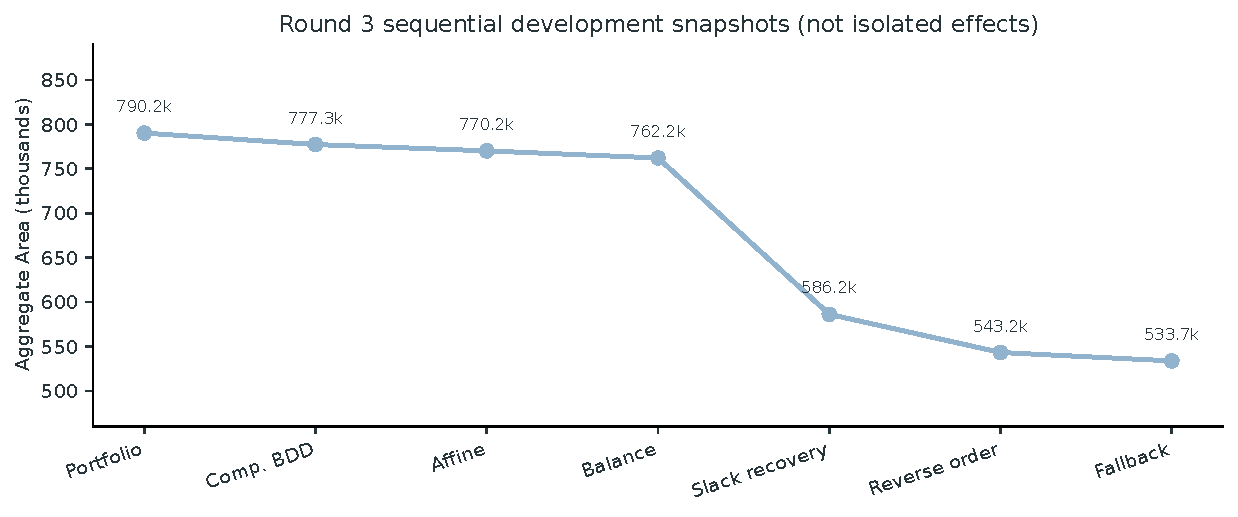
\includegraphics[width=.76\textwidth]{../shared/figures/round3_ablation_path.pdf}
\caption{Round 3 archived sequential development snapshots. Areas are historical full-program evaluator results; the isolated contribution of each module cannot be read causally from this line.}
\label{fig:r3ablation}
\end{figure*}

\subsection{Global phase choices and algebraic factoring}
Round 4 introduces a phase bit $p_v$ for an intermediate Boolean function $f_v$, allowing its stored realization to compute $g_v=\neg^{p_v}f_v$. When a node changes phase, De Morgan's laws interchange AND/OR while potentially moving or sharing NOT gates across fanouts. A coordinate-descent search estimates area for candidate phase assignments; actual DAG area and delay, rather than the surrogate, determine acceptance. A separate algebraic pass applies absorption and factoring identities such as
\begin{equation}
 (a\land b)\lor(a\land c)=a\land(b\lor c).
\end{equation}
A replacement that saves a standalone gate may still be worse globally because one old subexpression is shared elsewhere. Write $L(G)$ for the \emph{set} of gate IDs reachable from at least one output. Since shared gates are charged only once,
\begin{equation}\label{eq:livegain}
 A(G)=\sum_{v\in L(G)}a_{\operatorname{op}(v)},\quad
 \Delta A=A(G)-A(G').
\end{equation}
A gate in the rewritten cone is actually removed only if it loses \emph{all} paths to every output; conversely, a candidate may reuse an existing gate without paying for another copy. This is why a standalone expression's gate count cannot serve as the exact rewrite gain. All finalized candidates are pruned and remeasured. Round 4 lowered area but increased synthesis time, motivating the following engineering phase.


\subsection{Round 4 postprocessing ablation}
The Round 4 postprocessing record contains per-case areas for the original Round 3 circuits and five ways of selecting algebraic and phase rewrites. Summing the 25 input cases yields $533{,}705$ (original), $532{,}416$ (algebra only), $533{,}378$ (phase only), $532{,}078$ (phase then algebra), and $532{,}080$ (algebra then phase). Choosing the lowest tested area separately for each case yields $532{,}070$, a saving of $1{,}635$ against the original circuit set. The best-per-case result is a selector over recorded strategies, not one uniform transformation order. Most importantly, \emph{these numbers exclude the later variable-order exploration}: the complete Round 4 candidate reached $528{,}910$ on its archived Stage 1 run. This distinction prevents wrongly attributing the whole Round 3-to-4 improvement to the two local postprocessors.
\begin{figure*}[!t]
\centering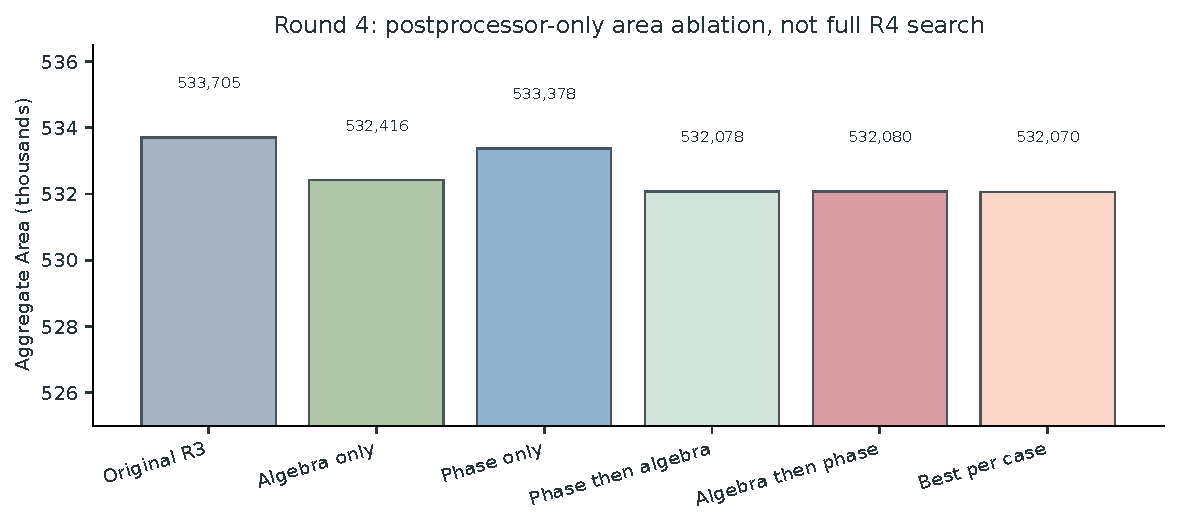
\includegraphics[width=.76\textwidth]{../shared/figures/round4_postprocess_ablation.pdf}
\caption{Round 4 postprocessor-only comparison, aggregated from the original 25-row ablation CSV. The horizontal axis distinguishes alternative treatment orders and a per-case minimum; this is not the complete R4 variable-order portfolio.}
\label{fig:r4ablation}
\end{figure*}

\section{A More Efficient Synthesis Engine}
The area improvements of Rounds 3--4 exposed a different bottleneck. More candidates or more local rewrite passes can reduce circuit cost, but also consume the finite time available for synthesis. We therefore changed the optimization target of the \emph{program itself}: first eliminate identical work, then reduce representation overhead, instead of immediately removing potentially useful search candidates. The empirical claim to test is lower synthesis time with unchanged completed-candidate semantics, not a new Boolean identity.
\subsection{Reuse without changing fixed-candidate semantics}
Let $B(F,\pi)$ denote a completed reduced BDD for the input table and a fixed variable order $\pi$; let $M(B,\theta)$ map that graph under one candidate configuration $\theta$. Several portfolio members reuse the same $\pi$. In Round 5, we build $B(F,\pi)$ once and share it read-only:
\begin{equation}
 C_i=M(B(F,\pi),\theta_i),\qquad i=1,\ldots,k.
\end{equation}
If a build costs $T_B$ and mapping candidate $i$ costs $T_{M,i}$, the repeated-build contribution $kT_B+\sum_iT_{M,i}$ becomes $T_B+\sum_iT_{M,i}$, at the cost of retaining one BDD in memory. This does not promise a large total speedup if gate mapping dominates. Small-support symbolic implicant covers are cached separately; only their gate realization depends on the candidate. A candidate differing solely in an inactive cube-generation flag is removed for $n>13$. The netlist cost parser is also replaced with a linear scanner.

\subsection{Typed DAG and incremental arrival propagation}
Round 5.1 replaces intermediate strings inside rebalancing and area recovery with a compact typed graph. A gate is stored as $(\mathrm{op},a,b)$ and new nodes are hash-consed. Its arrival time is computed on insertion from (\ref{eq:arrival}); topological construction makes this stored value exact. Repeated parsing and serialization are avoided across the principal rebalancing and recovery passes. A shared gate is identified by its operation and normalized input IDs. For AND2/OR2, the input order is canonicalized because these operations are commutative. Rebalancing flattens associative cones only across unshared interior gates (or the cone root); fanout references from \emph{all} outputs participate in the reference counts. For each old node $v$, topological induction shows that the mapped node implements the same function: the rewrites use associativity, commutativity and idempotence, while hashing reuses a gate only for identical operands and type. The builder traces all $m$ output roots, removes unreachable gates, and renumbers surviving nodes in topological order, preserving both functionality and output ordering. Area recovery uses exact De Morgan identities; its completed candidates are again evaluated over the reconstructed graph. Importantly, the implementation \emph{does not} perform fully incremental global-area evaluation: after rewriting, it recomputes area over the output-reachable emitted DAG, since shared fanout can make local area differences misleading.

\begin{proposition}[Typed-graph transformation and output preservation]
Suppose an input netlist is a valid topologically ordered AND2/OR2/NOT DAG. If the typed builder (i) creates only gates whose predecessors are already defined, (ii) replaces subgraphs using exact Boolean identities, (iii) shares nodes only when their operator and canonicalized operand IDs match, and (iv) serializes only gates reachable from the \emph{complete ordered list} of outputs, then its emitted netlist implements the same output vector as the input. For the emitted live graph, gate-count area and the arrival recurrence in (\ref{eq:area})--(\ref{eq:arrival}) are exact under the given library costs.
\end{proposition}
\begin{IEEEproof}
Proceed in topological order. Primary signals retain their values. A new gate computes the stated AND, OR, or NOT of already correct predecessors; each permitted algebraic replacement is an identity, so the corresponding mapped value is unchanged. Canonicalizing operand order is valid for commutative binary operators. Interning an identical operator/operand tuple reuses a node with exactly the same computed value. Finally, output-root reachability includes \emph{all} uses of shared gates; removing nodes outside this union cannot affect any output. Renumbering retained nodes in their original topological order preserves all predecessor references and leaves the ordered output vector unchanged. Each retained physical gate appears exactly once in the resulting graph, giving the stated area, while forward topological evaluation gives exact arrival times.
\end{IEEEproof}
This is a conditional structural argument, not an automated proof of every implementation detail. It does not establish that arbitrary nonlocal graph transformations preserve acyclicity or that a locally cheaper expression reduces the global area. The archived independent checks test the actual serialized implementation in addition to these mathematical conditions.

The frozen implementation compares candidates using an \emph{internal heuristic}, not an inferred evaluator score. For each valid netlist $G$, define
\begin{equation}\label{eq:rank}
\begin{split}
\rho(G)=\big(&\max\{0,D(G)-D_{\rm target}\},\\
&\mathbf1_{D(G)\le D_{\rm target}}A(G),\ D(G),\ A(G)\big).
\end{split}
\end{equation}
ordered lexicographically. In the feasible set, this ranks area before delay; for a target miss, delay excess comes first (and area is a later tiebreaker). The program also uses clock-based eligibility for candidates. The main loop checks elapsed time before later candidates, the legacy fallback has a separate cutoff, and final algebraic/phase passes have additional budget gates. Some extra BDD orderings use periodic internal deadline checks, but many stages are not preempted at every operation: these are \emph{soft search budgets}, not a proven hard wall-clock bound. Because the eligible set of completed candidates may change with machine speed or scheduling, the chosen answer can vary with execution environment without any change to Boolean identities. Within any one execution, a valid incumbent is updated only on strict lexicographic improvement; in particular, once a delay-feasible incumbent exists, no delay-infeasible candidate can replace it. The final netlist must still be checked by the official evaluator for functionality and resource limits.
\begin{algorithm}[t]
\caption{Frozen Round 5.1 control-flow overview}\label{alg:synth}
\begin{algorithmic}[1]
\Require Complete truth table $F$, gate costs, target, optional time limit
\State Parse input; initialize BDD/implicant caches
\State $C^*\gets\bot$ \Comment{no incumbent yet}
\For{each eligible modern mapping policy $\theta$}
  \State Map $F$ to an AND2/OR2/NOT netlist, using caches
  \State Parse into typed DAG; compute exact candidate metrics
  \State Try rebalancing; accept locally if $\rho$ improves
  \If{candidate meets target delay}
     \State Try required-time area recovery; remeasure
  \EndIf
  \If{valid and $(C^*=\bot$ or $\rho(C_\theta)<\rho(C^*))$}
     \State $C^*\gets\textsc{Serialize}(C_\theta)$
  \EndIf
\EndFor
\State Try budget-eligible legacy candidates; update $C^*$ by $\rho$
\State $B\gets C^*$ \Comment{freeze base for final postprocessing}
\If{time budget permits}
  \State Try algebraic rewrite of $B$; compare complete netlist
  \State Try phase mappings of $B$ and algebraic follow-ups
  \State Keep only candidates that improve $\rho(C^*)$
\EndIf
\State Emit the chosen topologically ordered netlist $C^*$
\end{algorithmic}
\end{algorithm}

Algorithm~\ref{alg:synth} follows the frozen control-flow hierarchy: typed rebalancing/recovery occur per mapping candidate, whereas the Round 4 algebra/phase alternatives are considered only after portfolio/legacy candidate selection. The dead-code guarded reverse-order phase branch is not claimed as executed. The frozen source is the authoritative implementation. A search decision can be wall-clock-dependent. Thus a faster implementation preserves the function of each fixed candidate but may complete a different candidate set by the cutoff, a distinction visible in an earlier container rerun of one case.

\subsection{What the in-memory improvement actually covers}
The typed graph is used inside the primary per-candidate balancing and area-recovery sequence. The final algebraic/phase alternatives still operate through serialized text and their own parsers. The internal typed parser is designed for netlists produced by the synthesizer; it is not presented as a complete adversarial-input validator, and structural correctness checks do not replace truth-table equivalence checking. Consequently ``in-memory'' is a statement about a \emph{specific high-frequency pipeline}, not an end-to-end text-free synthesizer. The runtime changes are empirical constant-factor gains; the truth-table input lower bound and worst-case BDD/cut complexity remain exponential.

\subsection{Why the efficiency baseline was frozen}
The selected R5.1 implementation has aggregate published-case area $529{,}014$, whereas the designated R4.1 Strict archive records $528{,}910$ (a difference of $104$, or about $0.020\%$). These are \emph{different engineering points}, not an area dominance result. R5.1 preserves all published delay targets and reduces processing overhead relative to its R5 predecessor in the two paired WSL runs reported below. No numerical course score has been disclosed, so the preference for R5.1 is an explicit reproducibility/efficiency decision and cannot be presented as a proven grade-maximizing choice. In particular, historical runtime observations from separate R4.1 and R5.1 archives are not a controlled paired speedup estimate.


\section{Exploration Beyond the Adopted Candidate}
After the efficiency refactor, we asked a different question: did the BDD-origin mapping leave locally equivalent gate structures unexplored? This experiment examines circuit quality rather than repeated-computation overhead. Round 6.0 enumerates up to four boundary signals for an internal node, simulates its cut function as a mask of at most $2^4=16$ bits, and generates exact alternative SOP, complemented SOP/POS, factored, and Shannon realizations. A $k$-feasible cut $C$ of root $v$ is a set of at most $k$ boundary signals intersecting every path from any primary input to $v$; the signals can therefore be treated as formal inputs for the local cone. For a cut $C$ at $v$,
\begin{equation}
 M_{v,C}=\sum_{s=0}^{2^{|C|}-1} f_{v,C}(s)\,2^s.
\end{equation}
For the running example, taking $(a,b,c)$ as the cut of output $f_2$ and indexing assignments in binary order $000,\ldots,111$ yields the local mask
$M=2^1+2^2+2^3+2^6+2^7=206$. Both $f_1\lor b$ and $b\lor(\neg a\land c)$ realize this mask. The second expression can bypass a slow output-to-output dependency, although it need not save area.
The leaves are \emph{formal} independent variables for enumeration, not asserted independent random variables. The local implementation is considered only if it is equivalent on every boundary assignment; the whole emitted DAG is then rescored. Equivalence on \emph{all} formal cut assignments is a sufficient substitution condition even when the boundary signals are correlated in the original circuit, because the actual assignment set is a subset of the tested formal assignments. It is not by itself sufficient for legal substitution if the rewrite adds a dependency cycle, changes external interfaces, or violates the gate library. Thus a valid rewrite must also preserve acyclicity and output connectivity. Its true area gain is given by the live-node accounting in (\ref{eq:livegain}), not by counting gates in the new cone alone. This is inspired by well-established cut-based logic rewriting approaches~\cite{mishchenko2006,abc}, but the project implementation uses a limited heuristic candidate set, not an exhaustive NPN rewrite database.

Round 6.1 reuses symbolic prime-implicant covers under a key $(|C|,M,p)$, prioritizes cuts by potentially removable private subgraph area, and restricts postprocessing to a 25 ms per-invocation cut budget (subject to a second budget depending on the case limit). A 25 ms \emph{postprocessor} budget does not mean that total synthesis runtime is 25 ms. Both stages are exact-function transformations, yet their search and area improvements are heuristic. The separate experiments show modest public-case area savings at a significant runtime cost, so Round 5.1 remains the adopted efficiency baseline.


\subsection{Round 6.1 development-budget evidence}
For the \emph{larger development set of 16 generated functions}, the archived cut-postprocessor study records local area saved of $358$, $408$, and $501$ at nominal search budgets of $25$, $35$, and $45$ ms, with corresponding median postprocessor wall times $31.66$, $40.89$, and $52.38$ ms (Fig.~\ref{fig:budget}). The 40-function mixed development set records $213$ area saved at each budget, with medians $4.84$, $4.59$, and $4.91$ ms, respectively. This contrast supports a workload-dependent diminishing-return analysis; it does \emph{not} supply 25-case official final Area, and these development sets must not be presented as previously unseen holdouts. The ultimately selected 25 ms budget is a local engineering choice, not a proof of optimality.
\begin{figure}[t]
\centering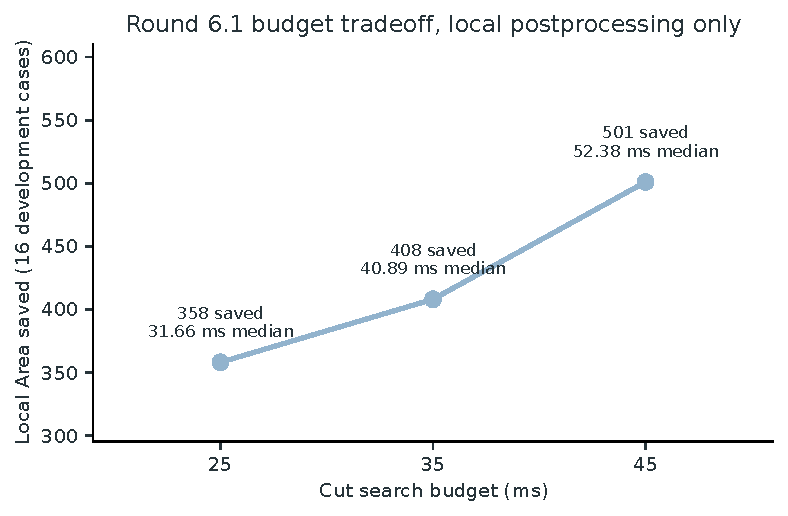
\includegraphics[width=\columnwidth]{../shared/figures/round61_budget_tradeoff.pdf}
\caption{Round 6.1 local cut-search budget study on 16 larger \emph{development} functions. Annotations give local median wall time; neither axis reports the full official Stage 1 synthesizer runtime.}
\label{fig:budget}
\end{figure}

\section{Experimental Methodology and Results}
\subsection{Protocol and scope of inference}
Our experimental argument has three distinct stages: establish a correct legal circuit, compare its measured cost with an appropriate baseline, and decide whether the gain is worth the additional synthesis work. A proof of a Boolean identity addresses the first stage but cannot establish the second; a smaller area total cannot, by itself, establish the third. We therefore report status, deadline feasibility, area and runtime separately, and reserve same-run paired measurements for runtime claims.

We evaluated archived source snapshots using the course Linux x86 evaluator. For each published case we record the official status, whether the target was met, circuit area, circuit delay, and measured synthesis runtime. Independent simulation checks gate legality and Boolean functions; small cases were exhaustively enumerated while larger cases used deterministic sampling in the independent checker. The official evaluator is the primary full-case correctness reference. We also ran generated structure families to probe regressions. We do \emph{not} infer unseen Stage 2 performance or claim that local wall-clock runtime is identical to a designated grading server.

\subsection{Supplementary test generation and evaluation protocol}
The published Stage 1 instances were the main development benchmark; supplementary instances were constructed by deterministic generators to test different Boolean structures and sizes. Each retained generator specifies a seed, the number of inputs $n$ and outputs $m$, per-gate area/delay costs, a delay target, and the truth bits of every output for all $2^n$ assignments. The accompanying manifests record input-file SHA-256 values. Sampling a Boolean-function \emph{family} is distinct from sampling independent truth bits: affine, sparse-SOP, threshold, multiplexor, arithmetic, shared-cone, small lookup-table, and seeded gate-DAG functions exercise different kinds of regularity and sharing.

For Round 5.1, the separately archived scripts specify $80$ mixed functions ($4\leq n\leq15$ in the generator, with family-specific caps, mostly $1$--$4$ outputs), and $16$ larger structured functions ($n\in\{12,14,16,17\}$; $m\in\{8,10,12,14\}$). A preexisting $110$-case suite and two stress cases serve as \emph{regression} evidence rather than fresh holdouts. In Round 6.1, after the selected cut budget was fixed, a new seeded $40$-case mixed suite ($8\leq n\leq13$, $3$--$5$ outputs) and an $8$-case larger suite ($n\in\{12,14,16,17\}$) were evaluated. The 25/35/45-ms budget sweeps used \emph{development} functions and are explicitly excluded from the independent-holdout claim.

Each generated instance is evaluated under the same legal netlist and Boolean-equivalence contract as an official case, but with its own chosen costs and target. We compare each candidate against the frozen comparator on identical instances, separating correctness, target satisfaction, area, delay, and runtime. A seeded holdout reduces reuse of the published cases, but does not estimate performance on the unknown Stage 2 distribution. Moreover, fixed seeds and source manifests provide repeatability, not a statistical confidence interval or proof that selection effects are absent. The included \texttt{TEST\_SUITE\_PROTOCOL.md} documents exact generators, archived seeds, function families and the evidence role of each suite; original inputs are not republished in the paper archive.


Figure~\ref{fig:history} shows one designated WSL archive per round; these archives were not an interleaved experiment, so the plot supports an \emph{area evolution} story, not a causal cross-round runtime claim. For performance comparisons, Fig.~\ref{fig:paired} instead uses official CSVs from each same-run paired benchmark. Precise source ZIP names and member paths are retained alongside the CSV tables in the supplementary evidence manifest.

\begin{figure*}[!t]
\centering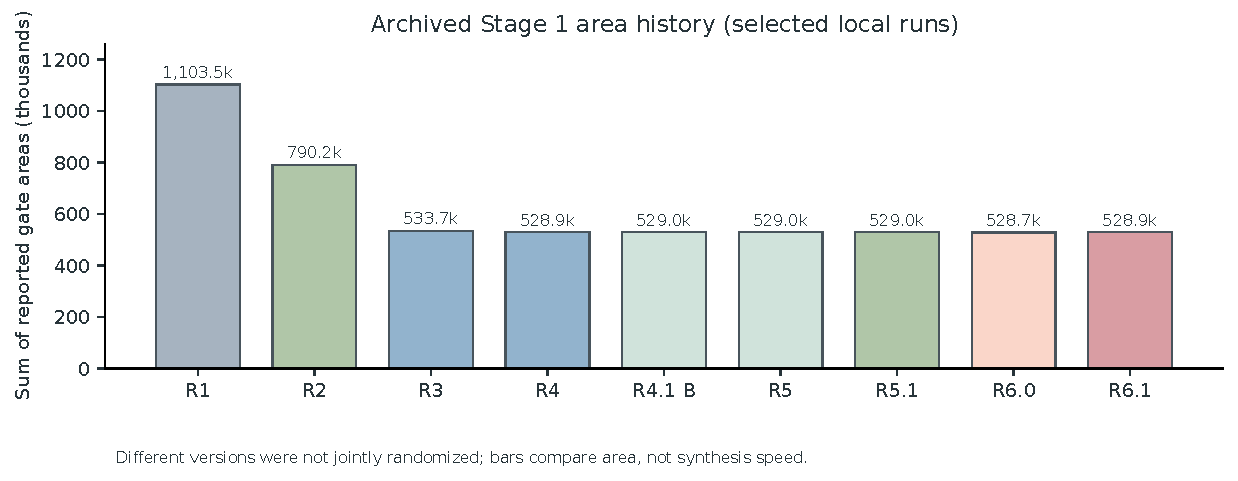
\includegraphics[width=.87\textwidth]{../shared/figures/area_evolution.pdf}
\caption{Circuit-area development across selected archived local runs. Round 6.0 and 6.1 are research branches, not the adopted default. Aggregate area is a descriptive metric, not a published official grading score.}\label{fig:history}
\end{figure*}

\begin{figure*}[!t]
\centering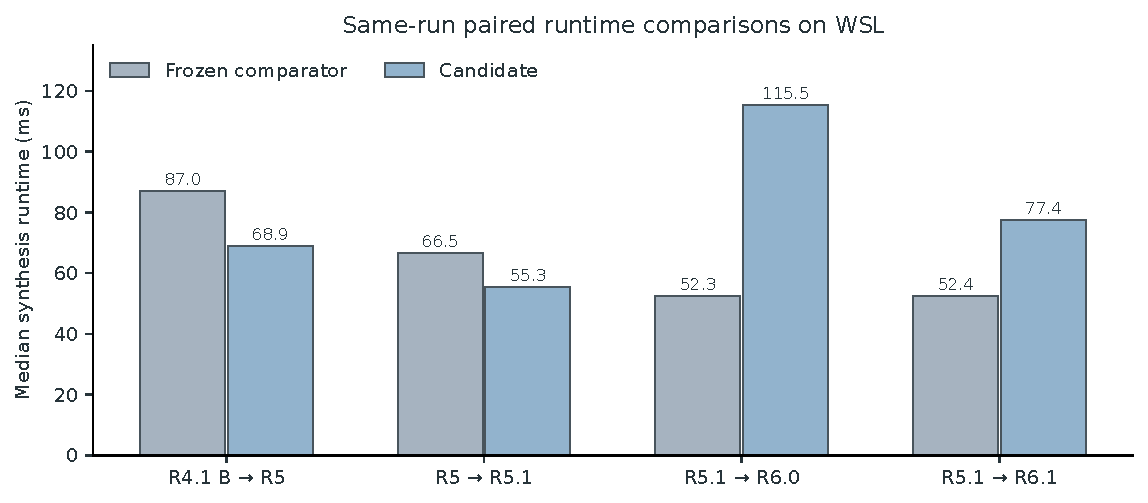
\includegraphics[width=.84\textwidth]{../shared/figures/paired_runtime.pdf}
\caption{Within-run WSL paired comparisons of median synthesis runtime. For comparisons having two paired runs, the plotted bar is the mean of the two per-run medians. Different comparison groups have distinct loads and cannot be interpreted as one continuous randomized experiment.}\label{fig:paired}
\end{figure*}

\begin{table*}[!t]
\centering\caption{Stage 1 milestones from individually archived WSL official-evaluator results}\label{tab:milestones}
\small\setlength{\tabcolsep}{11pt}
\begin{tabular}{@{}lccrr@{}}\toprule
Version & PASS & Target met & Area sum & Median synthesis runtime (ms) \\ \midrule
R1 baseline & 25/25 & 12/25 & 1,103,455 & 5.455 \\
R2 hybrid & 25/25 & 25/25 & 790,243 & 36.427 \\
R3 timed map & 25/25 & 25/25 & 533,705 & 68.486 \\
R4 polarity & 25/25 & 25/25 & 528,910 & 127.568 \\
R4.1 Balanced & 25/25 & 25/25 & 529,014 & 102.615 \\
R5 caching & 25/25 & 25/25 & 529,014 & 68.861 \\
\textbf{R5.1 typed DAG} & \textbf{25/25} & \textbf{25/25} & \textbf{529,014} & \textbf{55.488} \\
R6.0 cut proto. & 25/25 & 25/25 & 528,738 & 114.610 \\
R6.1 budgeted & 25/25 & 25/25 & 528,854 & 80.731 \\
\bottomrule\end{tabular}
\par\vspace{2pt}
\parbox{0.92\textwidth}{\footnotesize\emph{Comparability:} each row is one designated historical WSL run, not a randomized same-run comparison of every round. Runtime is the median of 25 official \texttt{runtime\_ms} values for that one archive; use Fig.~\ref{fig:paired} for directly paired runtime evidence. Values were not normalized across CPU loads.}
\end{table*}


Round 1 to Round 5.1 reduces aggregate area by 574,441, about 52.1\%, across the archived published-case results. The largest improvement occurs through representation diversification and timing-aware mapping (Rounds 2--3), rather than the later runtime refactors. The Stage 1 Round 5.1 official per-case result table is provided in Table~\ref{tab:fullcases}.


\subsection{Source freeze and a scoped resource observation}
The adopted \emph{research} baseline is the Round 5.1 source snapshot from WSL run \texttt{20261111\_134547\_Round5.1}. Its C++ entry point is \texttt{synth\_round51.cpp}; the complete SHA-256 digest is preserved in the bundled \texttt{raw\_evidence} freeze manifest. A student author independently checked the file digest on WSL and ran the evidence-collection script. This is a \emph{research freeze}, not a claim that this exact source has been submitted to Canvas.

A separate single-process GNU \texttt{/usr/bin/time -v} measurement on \texttt{case\_024} returned exit status 0, elapsed wall time $1.66$ s and maximum resident set size $69{,}480$ KiB ($67.85$ MiB); the synthesizer reported area $124{,}475$ and delay $70$. This result is transcribed from the student's terminal record, not independently reconstructed from a saved raw time log. The measurement is one process invocation, not an exhaustive peak-RSS bound over all cases and not a paired official-evaluator runtime. In particular, its nonzero netlist output alone does not establish correctness; that claim comes from the separately archived evaluator and independent checker.

\subsection{Same-run cost comparisons}
Round 5.1 was measured against frozen Round 5 twice on the same local WSL environment. The reference medians were 72.188 and 60.827 ms, and the typed-DAG medians were 55.488 and 55.077 ms, respectively. Both runs yielded 25/25 PASS, 25/25 targets, and area 529,014. In the first paired run the reported output files were byte-identical for all 25 cases. These are measured improvements, not an asymptotic theorem or a promise of proportional speedup on every input.

The cut-based branch demonstrates the opposite tradeoff. In two local Round 6.1 comparisons, the frozen Round 5.1 reference had median runtime 54.572 and 50.224 ms, whereas Round 6.1 took 80.731 and 74.083 ms. The candidate areas were 528,854 and 528,839 versus 529,014 for the reference. Thus the additional public-case area saving was only about 0.03\%, while the mean-of-medians runtime increased about 47.7\%, breaching our prespecified 30\% tolerance. Round 6.0 also improved area but at higher runtime cost. These findings motivate retaining R6.1 as a documented research prototype, not an unconditional upgrade.

\subsection{Beyond the public cases}
The Round 5.1 regression suites include 80 mixed synthetic functions, 16 larger structural cases, the preexisting 110 generated tests and two stress tests. Correctness checks passed; the older generated suite included target misses shared by both versions, which we do not mislabel as functional failures. For Round 6.1, the fresh frozen 40-case mixed and 8-case large sets passed both functionality and target delay. Their aggregate area changed from 11,186 to 10,858 and from 67,275 to 67,047, respectively, with higher median runtime in both sets. Synthetic holdouts test specific function families; they do not establish representativeness of future Stage 2 inputs.

\begin{figure}[!t]
\centering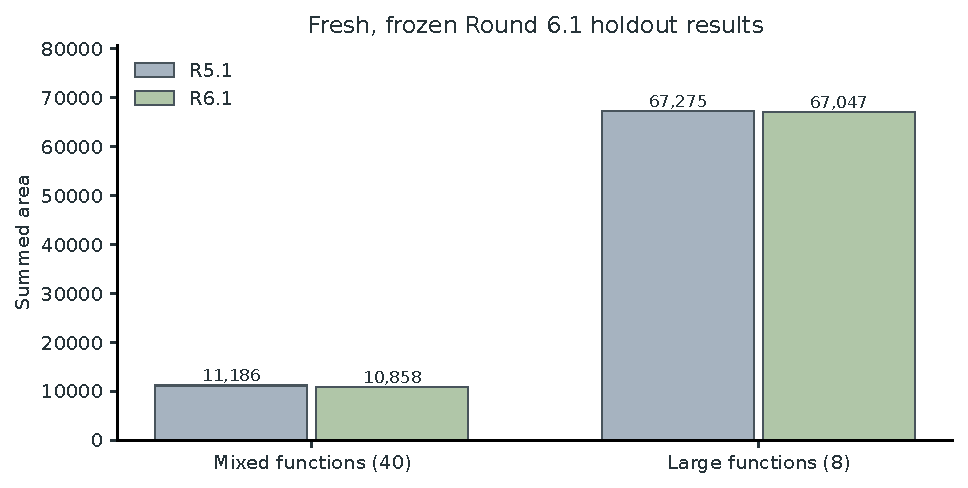
\includegraphics[width=\columnwidth]{../shared/figures/holdout_area.pdf}
\caption{Fresh Round 6.1 generated holdout groups. Lower area accompanies higher synthesis cost; source: paired CSVs archived with the experiment.}\label{fig:holdout}
\end{figure}

\section{Research Reproducibility and Source Provenance}

\subsection{A tiered reproduction protocol}
The phrase \emph{reproducible results} has several meanings, and we distinguish them by what materials are required. First, the seven published plots can be regenerated entirely from the intermediate CSVs shipped with the writing package; this tests plotting logic, \emph{not} the synthesis algorithm. Second, the selected official metrics can be re-extracted from the nine original, separately archived local-results ZIPs. We repeated this extraction during the manuscript audit: all 14 regenerated official, paired, summary and holdout CSV files matched the bundled normalized CSVs byte for byte. The archive SHA-256 digests and exact CSV members are recorded in the machine-readable \texttt{source\_manifest.csv}. The reproduction script validates the complete 25-case identifier set, numeric metrics and status fields; it does not infer unpublished official grades.

Third, the adopted algorithm source is separately frozen. The primary Round 5.1 entry-point SHA-256 starts with \texttt{cf90d0b1} and ends with \texttt{783e20759}; the complete digest, dependent headers, and archived source files are specified in the bundled freeze manifest. Recompiling and rerunning this source requires the designated Linux x86 environment, instructor-provided inputs and evaluator, and the archived build configuration. The writing ZIP intentionally does \emph{not} redistribute the private truth tables, evaluator binary or large netlists. It therefore supports self-contained \emph{figure reproduction} but not a self-contained rerun of the instructor's evaluation.

\begin{table}[!t]
\centering\footnotesize\setlength{\tabcolsep}{3pt}
\caption{Evidence reproduction levels and their inputs.}\label{tab:reprotier}
\begin{tabularx}{\columnwidth}{@{}p{.25\columnwidth}X@{}}\toprule
\textbf{Reproduction level} & \textbf{Needed inputs and what is checked}\\\midrule
Mathematical example & Bundled verification script; exhaustively rechecks the eight-row example.\\
Figures & Bundled normalized CSVs, plotting code and palette; re-renders vector/raster figures.\\
Historical metrics & Separate archived local-run ZIPs; re-extracts official CSVs and compares exact bytes.\\
Full official rerun & Frozen sources, instructor cases/evaluator, build system and Linux x86; generates a new measurement requiring fresh verification.\\\bottomrule
\end{tabularx}
\end{table}

\noindent The bundled \texttt{verify\_provenance.py} checks the shipped schema and raw-evidence hashes without external data. With the original run archives supplied, it also verifies archive digests and exact reconstructed tables; with the separate frozen-source directory it verifies all recorded source hashes. \emph{No result for a future evaluator rerun is asserted by these checks.} Since candidate eligibility uses elapsed wall time, source-level reproduction need not imply byte-identical output or equal runtime on different systems. Independent functional checking remains a distinct step after evaluation.

% Balance the last double-column discussion page before the single-column appendices.
\balance
\section{Discussion, Threats to Validity, and Conclusions}
\textbf{What changed the research direction?} Three observations governed the sequence. First, Round 1's 13 missed delay targets showed that exactness does not imply a useful gate architecture; this justified representation diversification. Second, the large area reduction around Round 3's required-time development path showed the importance of optimizing a shared graph under a global deadline, while the sequential nature of that record precludes isolated causal attribution. Third, the small public-case area gains and large synthesis-time penalties of the cut branch motivated a predeclared stopping rule, not another unbounded parameter sweep.

\textbf{Why freeze Round 5.1?} The adopted candidate is a deliberately chosen engineering point, not the minimum-area archived branch. R4.1 Strict is $104$ area units smaller, but the available runtime records for those versions are not paired; R5.1's measured efficiency advantage is established instead against R5. The cut-based R6.1 branch saves slightly more area but violates the predeclared local runtime tolerance. Because the grading formula is unavailable, this stopping decision is explicit and revisable rather than a claim of score optimality.

We distinguish four levels of evidence. A Boolean-identity proof is universal for the stated local transformation, but it does not automatically prove that its C++ implementation satisfies the transformation's preconditions. For example, a correct rewrite of a root may be wired incorrectly to an output, and a locally smaller cone may contain externally shared gates. Structural invariants, emitted-netlist verification and whole-network recomputation close different parts of this gap. Boolean identities and structural inductions prove function preservation for correctly applied transformations. Gate parsing, topological invariants and full-DAG rescoring address implementation correctness. The official evaluator and independent simulator provide empirical checks of emitted circuits. Finally, comparisons over released and synthetic instances support \emph{measured} performance findings. No level proves global minimum-area synthesis for arbitrary functions, optimal search under deadline constraints, or success on unseen case distributions.
\begin{table}[!t]
\centering\footnotesize\setlength{\tabcolsep}{3pt}
\caption{What each evidence layer establishes---and does not.}\label{tab:claimscope}
\begin{tabularx}{\columnwidth}{@{}p{.27\columnwidth}X@{}}\toprule
\textbf{Evidence} & \textbf{Permitted inference}\\\midrule
Identity / DAG proof & Function preservation under stated preconditions; not area optimality.\\
Evaluator / checker & Correctness of evaluated netlists and observed constraints; not all possible inputs.\\
Paired benchmark & Runtime and cost differences on that machine and run; not a universal speedup.\\
Synthetic holdout & Regression evidence for sampled families; not future Stage 2 distribution.\\\bottomrule
\end{tabularx}
\end{table}

The main lesson is that \emph{reusable structure and global constraints matter at different points}. An ROBDD removes identical Boolean subproblems; alternative mappings explore equivalent representations; required-time propagation makes timing slack available for area recovery; and typed-DAG engineering reduces overhead that would otherwise obscure the value of further search. Conversely, cut-based rewriting demonstrates that finding additional correct optimizations is not sufficient: their execution cost must also justify adoption.

For the Stage 1 source candidate we recommend freezing Round 5.1 until an actual submitted source snapshot is designated. Round 4.1 Strict is an area-oriented comparison and R6.0/R6.1 remain exploratory branches. The authorship and use of AI assistance are disclosed below; specific individual ownership of unverified implementation modules is not asserted. Stage 2 is out of scope of this Stage 1 manuscript.


\section{Collaborative Development and AI Assistance}
\label{sec:disclosure}
\textbf{Team contributions.} Jincan LI and Zeyun DU initially explored synthesis strategies independently, then compared alternatives and integrated selected methods into a common framework. Roles evolved through discussion and review rather than a fixed assignment of modules; we do not assert unverified individual ownership of code, proofs, or experiments.

\textbf{AI assistance.} Generative AI, principally ChatGPT, was used to suggest algorithms, generate and revise substantial C++ code, construct test, benchmark, data-collection and packaging scripts, and assist mathematical analysis and interpretation. This went well beyond language polishing. The student team directed and questioned research priorities and adoption decisions; a student author independently ran the official evaluator and local reproduction checks in WSL and verified the frozen source hash. AI-produced outputs were assessed against mathematical conditions, actual program behavior, evaluator evidence, and additional tests, without treating AI suggestions as authoritative. These checks do not prove global optimality or unseen-case success. The student authors accept responsibility for the accuracy, citations and integrity of the report.

\clearpage
\onecolumn
\appendices
\section{Full Stage 1 Official Results for the Adopted Candidate}
\begin{table}[!h]
\centering
\caption{Round 5.1, archived paired WSL run 1 (25 released cases). The evaluator records synthesis runtime in milliseconds.}\label{tab:fullcases}
\small\setlength{\tabcolsep}{12pt}
\begin{tabular}{@{}lcrrrc@{}}\toprule
Case & Status & Area & Delay & Runtime (ms) & Target met \\ \midrule
001 & PASS & 61,952 & 62 & 516.040 & Yes \\
002 & PASS & 18,897 & 60 & 158.015 & Yes \\
003 & PASS & 24,251 & 56 & 193.997 & Yes \\
004 & PASS & 4,550 & 47 & 21.072 & Yes \\
005 & PASS & 700 & 31 & 28.198 & Yes \\
006 & PASS & 5,962 & 46 & 28.858 & Yes \\
007 & PASS & 78,042 & 71 & 733.507 & Yes \\
008 & PASS & 8,637 & 50 & 34.178 & Yes \\
009 & PASS & 14,584 & 46 & 55.488 & Yes \\
010 & PASS & 4,712 & 32 & 121.601 & Yes \\
011 & PASS & 464 & 33 & 27.847 & Yes \\
012 & PASS & 5,359 & 25 & 22.392 & Yes \\
013 & PASS & 11,252 & 60 & 79.956 & Yes \\
014 & PASS & 11,662 & 61 & 273.612 & Yes \\
015 & PASS & 33,374 & 64 & 307.922 & Yes \\
016 & PASS & 2,149 & 40 & 16.153 & Yes \\
017 & PASS & 440 & 22 & 7.747 & Yes \\
018 & PASS & 1,232 & 31 & 10.784 & Yes \\
019 & PASS & 5,319 & 57 & 102.606 & Yes \\
020 & PASS & 766 & 30 & 36.661 & Yes \\
021 & PASS & 28,104 & 60 & 514.703 & Yes \\
022 & PASS & 1,320 & 31 & 34.305 & Yes \\
023 & PASS & 125 & 22 & 7.991 & Yes \\
024 & PASS & 124,475 & 70 & 2453.455 & Yes \\
025 & PASS & 80,686 & 60 & 730.141 & Yes \\

\midrule
\multicolumn{2}{l}{All cases: 25/25 PASS} & \textbf{529,014} & -- & -- & 25/25 \\
\bottomrule\end{tabular}
\end{table}

\section{Reproducibility and Data Lineage}
The accompanying evidence archive retains the original Round 3 and 4 ablation CSVs, both Round 6.1 budget JSON files, the research-freeze SHA-256 manifest and the labeled terminal transcription for the single-case Peak RSS. Its plotting script regenerates the new ablation figures from normalized CSVs. The collaborative workflow and the substantive role of AI systems are described in the dedicated disclosure section. The writing archive retains: (i) selected official metric CSVs, (ii) source and original-run SHA-256 manifests, (iii) a source-linked evidence matrix, (iv) extraction, provenance-checking and plotting scripts, and (v) generated figure PDFs and PNGs. Original program sources and instructor test assets are held in separate, access-controlled archives. The extraction code checks that each selected official CSV has exactly 25 cases and all report PASS. It does not modify runtime values or impute missing cases. A re-analysis of complete historical runs requires the separately archived local-results ZIP files, which are not replicated inside this writing package to avoid duplicating large netlists. Compiling this paper uses IEEEtran and BibTeX with the \texttt{IEEEtran.bst} bibliography style; both manuscripts load the shared \texttt{references.bib}. The course handout is cited as privately distributed material and is not assigned an invented public URL.

\bibliographystyle{IEEEtran}
\bibliography{../shared/bibliography/references}
\end{document}
